\documentclass[12pt]{article}

\usepackage{fullpage}
\usepackage[spanish]{babel}
\usepackage{amsfonts} %for double trace letters
\usepackage{amssymb}
\usepackage{amsmath} %for special/unusual mathematical characters
\usepackage{eufrak} %for gothic letters
\usepackage{graphicx} %Image includer package
\graphicspath{{Images/}} %Image directory
\usepackage{xcolor}

\usepackage{multicol} %For writing text in columns
\setlength{\columnsep}{1cm} %Defines separation of columns

\usepackage{tcolorbox} %for boxes that enclose text
\usepackage{color}
\definecolor{myblue}{rgb}{.8, .8, 1}

\usepackage{empheq}

\newlength\mytemplen
\newsavebox\mytempbox

\makeatletter
\newcommand\mybluebox{%
    \@ifnextchar[%]
       {\@mybluebox}%
       {\@mybluebox[0pt]}}

\def\@mybluebox[#1]{%
    \@ifnextchar[%]
       {\@@mybluebox[#1]}%
       {\@@mybluebox[#1][0pt]}}

\def\@@mybluebox[#1][#2]#3{
    \sbox\mytempbox{#3}%
    \mytemplen\ht\mytempbox
    \advance\mytemplen #1\relax
    \ht\mytempbox\mytemplen
    \mytemplen\dp\mytempbox
    \advance\mytemplen #2\relax
    \dp\mytempbox\mytemplen
    \colorbox{myblue}{\hspace{1em}\usebox{\mytempbox}\hspace{1em}}}

% for theorems
\usepackage{amsthm}
 
\theoremstyle{definition}
\newtheorem{definition}{Definici\'on}[section]


\begin{document}
	\title{Propiedades de N\'umeros Complejos}
	\author{Breggia, Bruno M.}
	\date{}
	\maketitle
	
 Los N\'umeros Complejos... aquellos n\'umeros cuyo nombre les hace mala fama, pero son clara evidencia de c\'omo la necesidad es la madre de todo invento, o mejor dicho... propulsora de todo \textit{descubrimiento}, como lo son los hallazgos matem\'aticos. ?`Es la unidad imaginaria un n\'umero inventado? Y... s\'i, como todos los dem\'as. Como el 1, el 2, el 3.14, el $\frac{1}{3}$, pero se los cre\'o para modelar algo que va m\'as all\'a del alcance de la manipulaci\'on del hombre. All\'i, entre todos esos n\'umeros, agregaremos a la unidad imaginaria $i$, que como ver\'an, o mejor dicho, no ver\'an, no representa una \textit{cantidad}, sino una entidad meramente imaginaria, una abstracci\'on \textit{pura}. Por ello, s\'olo nos resta hecharnos para atr\'as y contemplar c\'omo este enriedo se arma solo... tratando de \textbf{entender.}
 
 Les damos la oficial bienvenida al mundo de \textit{las Variables Complejas.}\\
 \linebreak
	
	\begin{center}
		
\includegraphics[scale=0.5]{math_joke.png}
	\end{center}

\pagebreak

\tableofcontents

\pagebreak

\section{El n\'umero Complejo}

\colorbox{red!40!white!80}{\parbox{\linewidth}{
\theoremstyle{definition}
\begin{definition}{N\'umero Complejo}

 Un N\'umero Complejo se define como un par ordenado de n\'umeros reales: $$z = (x, y)$$
 
 Con $x, y \in \mathbb{R}$. La primer componente del par ordenado se denomina la \textbf{parte real} del n\'umero complejo, y se expresa como: $$\mathfrak{Re}(z) = x$$
 
 El segundo componente del par se denomina la \textbf{parte imaginaria} del n\'umero complejo, y la denotamos: $$\mathfrak{Im}(z)=y$$
\end{definition}
 }}
 \linebreak
 \linebreak
 
 El conjunto de \textbf{todos} los n\'umero complejos se designa con $\mathbb{C}$.
	\begin{empheq}[box={\mybluebox[5pt]}]{equation*}
		\mbox{ \large $\mathbb{C} = \{ (x, y): x \in \mathbb{R} \land y \in \mathbb{R} \}$}
	\end{empheq}

\section{Igualdad entre complejos: aclarando lo obvio}
Dos n\'umeros complejos son iguales si y s\'olo si sus partes reales e imaginarias son iguales entre s\'i. Dicho simb\'olicamente, si $z_1, z_2 \in \mathbb{C}$, entonces:
	\begin{empheq}[box={\mybluebox[5pt]}]{equation*}
		\mbox{ \large $z_1=z_2 \Leftrightarrow \mathfrak{Re}(z_1) = \mathfrak{Re}(z_2) \land \mathfrak{Im}(z_1) = \mathfrak{Im}(z_2)$}
	\end{empheq}
	\begin{center}
		
\includegraphics[scale=3]{Igualdad.jpg}
	\end{center}

\section{Operaciones Definidas en $\mathbb{C}$}
 Para poder hacer c\'alculos con estos nuevos n\'umeros, deberemos primero definir qu\'e operaciones ser\'an v\'alidas entre ellos, y c\'omo proceder en cada caso. Sabemos sumar n\'umeros reales, pero los complejos son tuplas, o pares ordenados. As\'i que damos lugar a nuestra imaginaci\'on para que abstraiga los conceptos de suma y multiplicaci\'on para poderlos aplicar con los elementos del conjunto $\mathbb{C}$.\\
 
 \colorbox{red!40!white!80}{\parbox{\linewidth}{
 \theoremstyle{definition}
 \begin{definition}{Suma de n\'umeros complejos}

   Con $z_1, z_2 \in \mathbb{C}$, tenemos que:
  $$z_1 + z_2 = (x_1, y_1) + (x_2, y_2) \triangleq (x_1+x_2 , y_1+y_2)$$ 
 
 \end{definition}}}
 \linebreak
 
 Con esto, la suma de n\'umeros complejos se define en t\'erminos de sumas de n\'umeros reales, y s\'i que sabemos sumar reales. Problema resuelto.\\
 
 \colorbox{red!40!white!80}{\parbox{\linewidth}{
  \theoremstyle{definition}
 \begin{definition}{Producto de n\'umeros complejos}

   Con $z_1, z_2 \in \mathbb{C}$, tenemos que:
  $$z_1.z_2 = (x_1, y_1)(x_2, y_2) \triangleq (x_1x_2 - y_1y_2 , x_1y_2 + x_2y_1)$$ 
 
 \end{definition}}}
 \linebreak
 
 Aqu\'i pareciese que la cuesti\'on se pone menos intuitiva, pero cr\'eanme que esto es por un bien mayor, que quedar\'a bien en claro cuando avancemos m\'as adelante y nos adentremos m\'as en el tema. En fin, el producto entre complejos se define en t\'erminos de productos y sumas entre reales, operaciones que ya sabemos realizar. Problema resuelto.\\
 
\subsection{Propiedades algebraicas}
	Se tiene que para $\forall z_1, z_2, z_3 \in \mathbb{C}$, se cumple que:
	\begin{enumerate}
		\item \textbf{Propiedad de Cierre}:
		\begin{empheq}[box={\mybluebox[5pt]}]{equation*}
			\mbox{ \large $z_1 + z_2 \in \mathbb{C}$}			
		\end{empheq}
		\begin{empheq}[box={\mybluebox[5pt]}]{equation*}
			\mbox{ \large $z_1z_2 \in \mathbb{C}$}			
		\end{empheq}
		
		\item \textbf{Propiedad Conmutativa}:
		\begin{empheq}[box={\mybluebox[5pt]}]{equation*}
			\mbox{ \large $z_1 + z_2 = z_2 + z_1 $}			
		\end{empheq}
		\begin{empheq}[box={\mybluebox[5pt]}]{equation*}
			\mbox{ \large $z_1z_2 = z_2z_1$}			
		\end{empheq}
		
		\item \textbf{Propiedad Asociativa}:
		\begin{empheq}[box={\mybluebox[5pt]}]{equation*}
			\mbox{ \large $(z_1 + z_2) + z_3= z_1 + (z_2 + z_3) $}			
		\end{empheq}
		\begin{empheq}[box={\mybluebox[5pt]}]{equation*}
			\mbox{ \large $(z_1z_2)z_3= z_1(z_2z_3) $}
		\end{empheq}
		
		\item \textbf{Propiedad Distributiva}: del producto respecto a la suma
		\begin{empheq}[box={\mybluebox[5pt]}]{equation*}
			\mbox{ \large $z_1(z_2 + z_3) = z_1z_2 + z_1z_3 $}			
		\end{empheq}			
		
		\item Existencia del \textbf{Elemento Neutro aditivo}:
		\begin{empheq}[box={\mybluebox[5pt]}]{equation*}
			\mbox{ \large $\exists! z\in \mathbb{C}\ /\ z_1 + z = z + z_1 = z_1 $}			
		\end{empheq}
		El elemento neutro aditivo $z$ resulta ser \'unico, y es el complejo $(0,0)$. De ahora en m\'as,su notaci\'on ser\'a equivalente a $z = (0,0) = 0$.
		
		\item Existencia de la \textbf{Identidad Multiplicativa}:
		\begin{empheq}[box={\mybluebox[5pt]}]{equation*}
			\mbox{ \large $\exists! z\in \mathbb{C}\ /\ z_1z = zz_1 = z_1 $}			
		\end{empheq}
		El elemento neutro multiplicativo $z$ resulta ser \'unico, y es el complejo $(1,0)$.  De ahora en m\'as, su notaci\'on ser\'a equivalente a $z = (1,0) = 1$.
		
		\item Existencia del Inverso Aditivo (\textbf{opuesto}):
		\begin{empheq}[box={\mybluebox[5pt]}]{equation*}
			\mbox{ \large $\forall z \in \mathbb{C}\ \ \exists! (-z) \in \mathbb{C}\ /\ z+(-z) = (-z)+z = 0$}			
		\end{empheq}
		Se dice entonces que $-z$ es el opuesto de $z$. Como la relaci\'on es rec\'iproca, podemos decir tambi\'en que $z$ es el opuesto de $-z$.
		
		\item Existencia del Inverso Multiplicativo (\textbf{rec\'iproco}):
		\begin{empheq}[box={\mybluebox[5pt]}]{equation*}
			\mbox{ \large $\forall z \in \mathbb{C}-\{0\}\ \ \exists! z^{-1} \in \mathbb{C}\ /\ zz^{-1} = z^{-1}z = 1$}			
		\end{empheq}
		Se dice entonces que $z^{-1}$ es el rec\'iproco de $z$. Como la relaci\'on es rec\'iproca, podemos decir tambi\'en que $z$ es el rec\'iproco de $z^{-1}$. 
		
	\end{enumerate} 
 
		
		\begin{center}
			
\includegraphics[scale=0.6]{Escriba.jpg}
		\end{center}
		De esta manera vamos construyendo, desde los cimientos hasta la cima, las bases y principios del c\'alculo con variables complejas, sobre los cuales nos respaldaremos a la hora de partir a realizar an\'alisis matem\'aticos m\'as avanzados. !`Bienvenidos a $\mathbb{C}$!
 
\subsection{Unas operaciones m\'as}
	Habiendo definido los opuestos y rec\'iprocos, nos vemos habilitados ahora a definir un par de operaciones m\'as, que son, por supuesto, an\'alogas a su contrapartida en el conjunto de los n\'umeros reales.\\
	
	\colorbox{red!40!white!80}{\parbox{\linewidth}{
 	\theoremstyle{definition}
 	\begin{definition}{Diferencia de n\'umeros complejos}

	   Con $z_1, z_2 \in \mathbb{C}$, tenemos que: $$z_1 - z_2 \triangleq z_1 + (-z_2)$$
	   Donde $-z_2$ es el opuesto de $z_2$.
	 
 	\end{definition}}}
 	\linebreak
 
	Con esto, !`la diferencia de n\'umeros complejos se define en t\'erminos de su suma!. Bien simple.\\
  
  \colorbox{red!40!white!80}{\parbox{\linewidth}{
 	\theoremstyle{definition}
 	\begin{definition}{Cociente de n\'umeros complejos}

	   Con $z_1, z_2 \in \mathbb{C}$, tenemos que: $$\frac{z_1}{z_2} \triangleq z_1(z_2^{-1})$$
	   Donde $z_2^{-1}$ es el rec\'iproco de $z_2$, con $z_2 \neq 0$.
	 
 	\end{definition}}}
 	\linebreak
 
	Con esto, el cociente de n\'umeros complejos se define puramente en t\'erminos de su producto. M\'as simplificado, imposible.\\
  
\section{Formas de representaci\'on}
Lleg\'o la hora de finalmente simplificarnos la cuesti\'on. Anotar n\'umeros complejos como pares ordenados puede resultar tedioso. No debemos confundirnos adem\'as con los puntos en $\mathbb{R}^2$, porque NO son lo mismo. Y encima multiplicar dos complejos entre s\'i ya es agarrarse la cabeza... o se sabe de memoria la definici\'on o se la debe tener por all\'i cerca. Por ello es que se han desarrollado m\'ultiples formas de representar ese par ordenado de tal forma que nos sea m\'as ameno operar con ellas, de diferenciarlos de puntos en $\mathbb{R}^2$ y de inclusive operar con ellos como si inconscientemente los trat\'aramos como n\'umeros reales. Es impresionante la importancia que tiene una buena forma de representaci\'on.

\begin{center}
	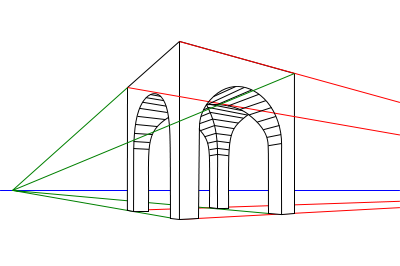
\includegraphics[scale=0.5]{Perspectiva.png}
\end{center}
 
\subsection{La Unidad Imaginaria y la Representaci\'on Binomial}
	Al n\'umero complejo $(0, 1)$ lo denominaremos la \textit{unidad imaginaria}, pues s\'olo posee la unidad como su parte imaginaria, y lo denotaremos con $i$ (la i de imaginario). Es decir,
	\begin{empheq}[box={\mybluebox[5pt]}]{equation*}
		\mbox{ \large $i = (0, 1) $}			
	\end{empheq}
Con esta definici\'on de $i$, todo n\'umero complejo se ve habilitado a escribirse como combinaci\'on lineal de los elementos $1=(1,0)$ e $i=(0,1)$, los cuales constituyen una base para el conjunto $\mathbb{C}$. Por si no me creen...
	\begin{eqnarray*}
		z = (x, y) &=& (x,0) + (0,y)\\
		&=& (1,0)(x,0) + (0,1)(y,0)\\
		&=& 1 \cdot (x,0) + i \cdot (y,0)\\
		&=& x + iy
	\end{eqnarray*}
 
 Llegamos a demostrar que con la definici\'on de la unidad imaginaria, todo n\'umero complejo puede representarse de forma binomial de la siguiente manera:
 	\begin{empheq}[box={\mybluebox[5pt]}]{equation*}
		\mbox{ \large $z = (x, y) = x+iy $}			
	\end{empheq}
	
Antes de continuar, vale la pena estudiar un poco m\'as detenidamente a la unidad imaginaria por s\'i misma, ya que fascinantes descubrimientos nos esperan.

Tomemos por ejemplo las potencias de la unidad imaginaria. Por convenci\'on respetaremos la regla de que todo n\'umero elevado al exponente 0 da como resultado 1. Con ello, $i^0=1$. Tenemos tambi\'en que $i^1=i$. Pero algo fuera de lo que estamos acostumbrados surge al calcular $i^2$:
\begin{eqnarray*}
	i^2 = (0,1)(0,1) &=& (0\cdot0-1\cdot1, 0\cdot1+0\cdot1)\\
	&=& (-1, 0)\\
	i^2 &=& -1
\end{eqnarray*}

Usando la definici\'on del producto (s\'i, esa f\'ormula complicada de la secci\'on anterior), demostramos que $i^2$ resulta en un n\'umero real, y no s\'olo eso, sino que da -1. Es como la pieza del rompecabezas que faltaba, al fin, un n\'umero que al elevarlo al cuadrado nos da algo... negativo. Se\~noras y se\~nores, aj\'ustensen los cinturones que esto reci\'en empieza.

Para avanzar algo m\'as r\'apido, les presento ya calculada una tabla de potencias de la unidad imaginaria:

\begin{multicols} {2}

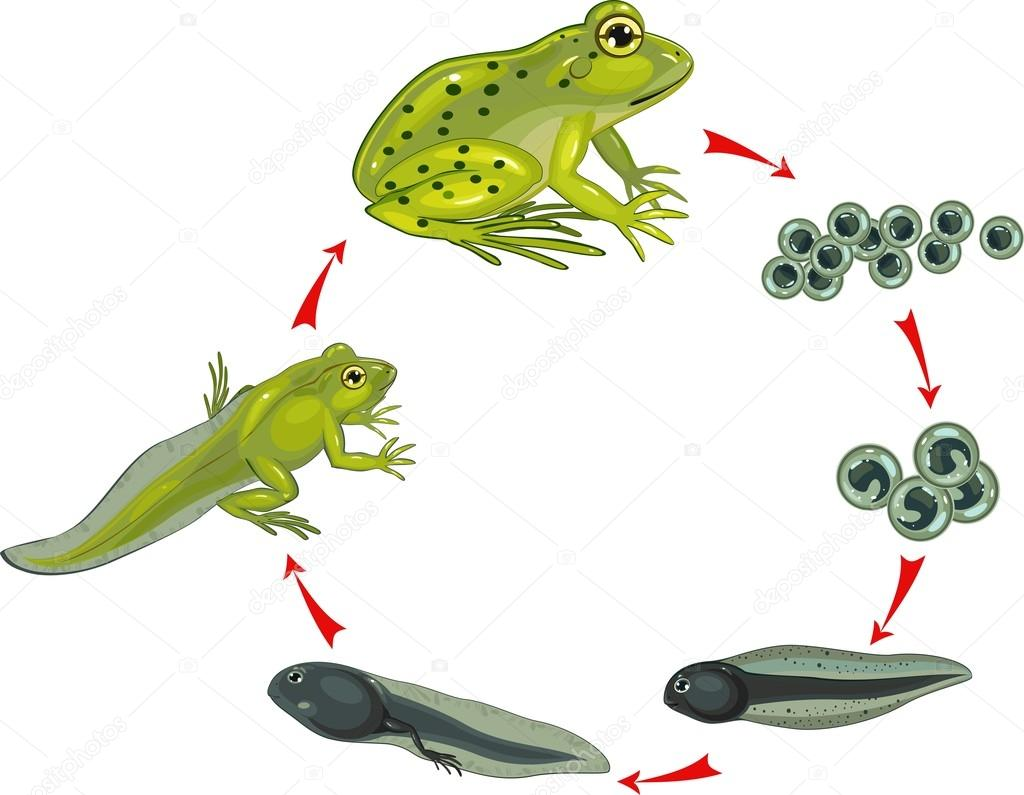
\includegraphics[scale=0.18]{ciclo.jpg}

\begin{center}
	\begin{tabular}{cc}
	Potencia & Valor\\
	\hline
	$i^0$ & $1$\\
	$i^1$ & $i$\\
	$i^2$ & $-1$\\
	$i^3$ & $-i$\\
	$i^4$ & $1$\\
	$i^5$ & $i$\\
	$i^6$ & $-1$\\
	$i^7$ & $-i$\\
	... & ...
	\end{tabular}
\end{center}

\end{multicols}

Obviamente, de los cuatro posibles valores podemos calcular cualquier potencia de $i$ simplificando el exponente: lo reemplazamos por el resto de su divisi\'on entera en 4, y calculamos la nueva potencia resultante. Esto es debido al car\'acter c\'iclico de las potencias de la unidad imaginaria.

La forma de representaci\'on binomial nos simplifica las operaciones algebraicas, pues operamos sobre los complejos como si fuesen n\'umeros reales, aplicando la propiedad distributiva, asociativa y conmutativa cuando corresponda.
Si $z_1, z_2 \in \mathbb{C}$, entonces...

\begin{empheq}[box={\mybluebox[5pt]}]{equation*}
		\mbox{ \large $z_1 + z_2 = (x_1 + iy_1)+(x_2 + iy_2) = (x_1+x_2)+ i(y_1+y_2)$}
\end{empheq}

\begin{empheq}[box={\mybluebox[5pt]}]{equation*}
		\mbox{ \large $z_1 - z_2 = (x_1 + iy_1)-(x_2 + iy_2) = (x_1-x_2)+ i(y_1-y_2)$}
\end{empheq}

\begin{empheq}[box={\mybluebox[5pt]}]{equation*}
		\mbox{ \large $z_1 z_2 = (x_1 + iy_1) (x_2 + iy_2) = (x_1x_2-y_1y_2)+ i(x_1y_2+x_2y_1)$}
\end{empheq}

\begin{empheq}[box={\mybluebox[5pt]}]{equation*}
		\mbox{ $\displaystyle \frac{z_1} {z_2} = \frac{(x_1 + iy_1)} {(x_2 + iy_2)} = \frac{(x_1x_2-y_1y_2)}{x^2+y^2}+ i\frac{(x_1y_2+x_2y_1)}{x^2+y^2}$}
\end{empheq}

Si te preguntas c\'omo hicimos para calcular esto \'ultimo, hemos partido de multiplicar numerador y denominador por el \textit{conjugado} de $z_2$...\\

 \colorbox{red!40!white!80}{\parbox{\linewidth}{
 \theoremstyle{definition}
 \begin{definition}{El Conjugado de un N\'umero Complejo}

   Con $z \in \mathbb{C}$, tenemos que el \textbf{conjugado} de $z$, denotado como $\bar{z}$, se define como:
  $$\bar{z} = \overline{x + iy} = x - iy$$ 
 
 \end{definition}}}
 \linebreak
 
 La conjugaci\'on no implica m\'as que cambiarle el signo a la parte imaginaria de un n\'umero complejo. Si no posee parte imaginaria (es real puro), entonces permanecer\'a igual.
\\
 
 Iremos creando m\'as definiciones a medida que nos sea necesario. Pero no nos olvidaremos de ninguna de las ya creadas a medida que vayamos avanzando.
 
\subsection{El Plano de Argand y la Representaci\'on Gr\'afica}
Lo hemos dicho una vez, y no est\'a dem\'as decirlo otra... un n\'umero complejo si bien es un par ordenado de dos n\'umeros pertenecientes a $\mathbb{R}$, no es un punto en $\mathbb{R}^2$. Sin embargo, hay una relaci\'on \'intima entre los n\'umeros complejos y los puntos en el plano $\mathbb{R}^2$, o mejor dicho, con los vectores en $\mathbb{R}^2$.

Entre las similitudes, ambos poseen dos componentes (reales), su suma se realiza componente a componente, el orden de sus componentes importa, son multiplicables por un n\'umero $\alpha \in \mathbb{R}$ y tienen opuestos definidos y un elemento neutro aditivo. Sin embargo, basta mencionar una y s\'olo una diferencia como para que caigamos en la realidad de que son elementos distintos (aunque realmente hayan m\'as diferencias): sus productos. Productos entre complejos nos da otro complejo que ninguna relaci\'on guarda con un vector producto, ya sea producto cruz o producto punto. Adem\'as, un complejo, como veremos m\'as adelante, tiene definido tambi\'en potenciaci\'on, ra\'ices, entre otras operaciones que a un vector no se les puede aplicar.

Pero gracias a lo poco que guardan en com\'un, nos es un incentivo para visualizar a los n\'umero complejos como puntos en un plano bidimensional, con su parte real e imaginaria como sus coordenadas. Es as\'i c\'omo organizamos a TODOS los puntos del conjunto $\mathbb{C}$ en un \textit{plano complejo}. Un plano cuyos ejes coordenados, an\'alogos a los ejes $x$ y $y$ de $\mathbb{R}^2$, son los ejes \textit{Real} e \textit{Imaginario}. Esto constituye el denominado \textbf{Plano de Argand}.

\begin{center}
	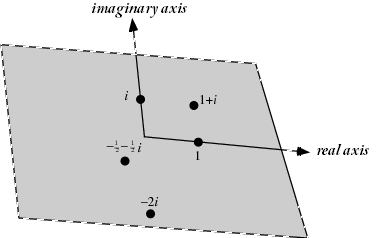
\includegraphics[scale=0.7]{Argand.png}
	\begin{center}
		El \textbf{Plano de Argand} o \textbf{Plano Complejo}
	\linebreak	
	\end{center}
\end{center}


\begin{multicols} {2}
	De esta manera, observamos c\'omo el eje real contiene a los n\'umeros puramente reales (con parte imaginaria 0), y el eje imaginario a los n\'umeros puramente imaginarios (con parte real 0). Lo contemplaremos al plano de Argand como una extensi\'on intuitiva de lo que conoc\'iamos como \textit{recta num\'erica}, contenida enteramente en el eje real de nuestro plano, lo cual tiene l\'ogica, ya que $\mathbb{R} \subset \mathbb{C}$.
	
	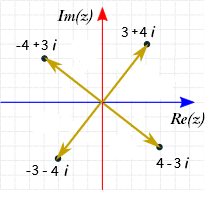
\includegraphics[scale=1]{Argand_plane2.png}
\end{multicols}

Esta representaci\'on nos hace notar el siguiente hecho fundamental:

\begin{empheq}[box={\mybluebox[5pt]}]{equation*}
		\mbox{ El conjunto $\mathbb{C}$ no es un conjunto ordenado}
\end{empheq}
 
 Es decir, no se define relaci\'on de precedencia alguna entre los elementos del conjunto de los n\'umeros complejos. Dados $z_1, z_2 \in \mathbb{C}$, podemos corroborar su igualdad o desigualdad, pero no si uno es mayor o menor que el otro. Al tratar con n\'umeros reales, todos pod\'ian ser ubicados en una recta infinita en la cual guardaban una relaci\'on de precedencia que nos permit\'ia compararlos entre s\'i seg\'un el orden en el cual los ubic\'abamos en la recta. Esto sin emabargo no es posible si hablamos de un plano con extensi\'on infinita.\\
 
Bueno, ni que lo anterior hayan sido malas noticias, la representaci\'on gr\'afica nos incentiva adem\'as a definir una nueva propiedad para los n\'umeros complejos, an\'aloga al m\'odulo de los vectores en $\mathbb{R}^2$, que representa la distancia de un n\'umero complejo $z$ al punto $z=0$ en el plano de Argand.\\

\colorbox{red!40!white!80}{\parbox{\linewidth}{
 \theoremstyle{definition}
 \begin{definition}{El M\'odulo de un N\'umero Complejo}

   Con $z \in \mathbb{C}$, tenemos que el \textbf{m\'odulo} de $z$, denotado como $|z|$, se define como:
  $$|z| = |x + iy| = \sqrt[2]{x^2 + y^2}$$ 
 
 \end{definition}}}
 \linebreak
 
 Tal definici\'on se basa en el teorema de pit\'agoras, tomando la parte real e imaginaria como si fuesen los componentes de un vector en $\mathbb{R}^2$ y calculando su m\'odulo. Sin embargo, cabe destacar que la distancia es una medida que ser\'a siempre un valor \textit{real} no negativo. Por lo tanto, el m\'odulo de todo n\'umero complejo $z$ tendr\'a que necesariamente tener su parte imaginaria igual a 0. !`Es una operaci\'on que, aplicada a cualquier complejo, nos garantiza obtener un n\'umero puramente real!
 
 Se puede establecer entonces una correspondencia biun\'ivoca entre los puntos del plano complejo $\mathbb{C}$ y $\mathbb{R}^2=\mathbb{R}\times\mathbb{R}$, dado un sistema de referencia cartesiano.
 
 \begin{center}
 	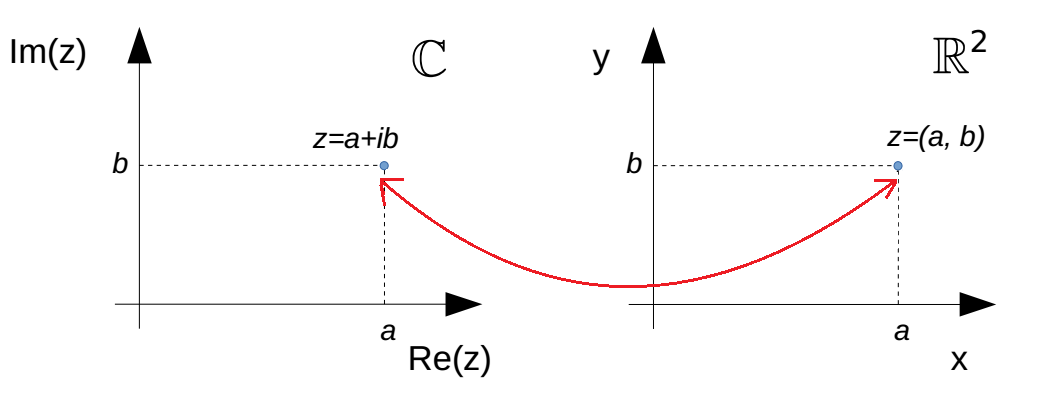
\includegraphics[scale=0.5]{correlacion.png}
 \end{center}
 
 Recordando la definici\'on del conjugado... podemos observar en el plano de Argand qu\'e interesante relaci\'on guardan entre s\'i los complejos conjugados. Calcular el conjugado de un complejo implica reflejar su representaci\'on gr\'afica respecto al eje real.
 
 \begin{multicols} {2}
	\begin{center} 
	 	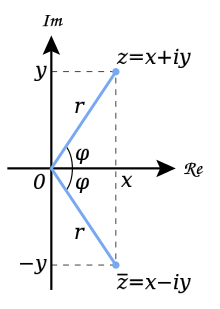
\includegraphics[scale=0.6]{conjugado.png}
	 	
\includegraphics[scale=0.4]{tree.jpg}
 	\end{center}
 \end{multicols}

\subsubsection{Propiedades del Conjugado y el M\'odulo}
Llegado a este punto, no avanzaremos sin antes introducir importantes propiedades a tener en cuenta a la hora de trabajar con m\'odulos y conjugados de n\'umeros complejos. Siendo que $z, z_1, z_2 \in \mathbb{C}$, se tiene que:

	\begin{enumerate}
		\item[a)] $z = \overline{\bar{z}}$
		\item[b)] $\overline{z_1 \pm z_2} = \overline{z_1}\pm \overline{z_2}$
		\item[c)] $\overline{z_1 \cdot z_2} = \overline{z_1}\cdot \overline{z_2}$\ \ y $\displaystyle \overline{\left(\frac{z_1}{z_2}\right)} = \frac{\overline{z_1}}{\overline{z_2}}$ con $z_2 \neq 0$
		\item[d)] $|\bar{z}| = |z|$
		\item[e)] $z\cdot\bar{z} = |z|^2$
		\item[f)] $|z_1 \cdot z_2| = |z_1| \cdot |z_2|$
		\item[g)] $\mathfrak{Re}(z) = \frac{1}{2} (z + \bar{z})$ e $\mathfrak{Im}(z)=\frac{1}{2i}(z-\bar{z})$
		\item[h)] $|z| \geq 0 \land |z|=0 \Leftrightarrow z=0$
		\item[i)] $\mathfrak{Re}(z)\ \leq\ |\mathfrak{Re}(z)|\ \leq\ |z|$ y $\mathfrak{Im}(z)\ \leq\ |\mathfrak{Im}(z)|\ \leq\ |z|$
		\item[j)] $|z^{-1}| = |z|^{-1}$
		\item[k)] Desigualdad Triangular: $|z_1 + z_2| \leq  |z_1| + |z_2|$
		\item[l)] Segunda desigualdad triangular: $\left| |z_1| - |z_2| \right| \leq  |z_1 - z_2|$
	\end{enumerate}

\subsection{La Representaci\'on Polar}
Dado el complejo $z=(x, y) \neq (0,0)$, podemos definirle \textbf{coordenadas polares} $r$ y $\theta$ tales que:

\begin{multicols} {2}
\begin{eqnarray*}
x &=& r\cdot \cos \theta\\
y &=& r\cdot \sin \theta 
\end{eqnarray*}
\linebreak

\begin{center}
	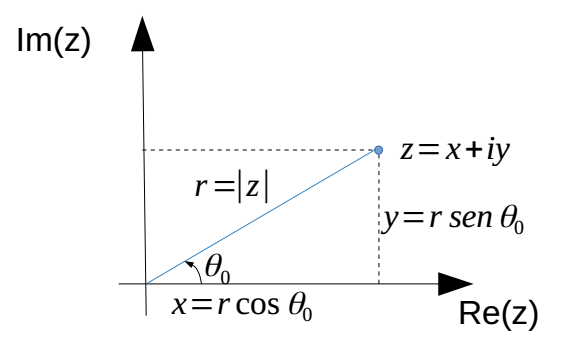
\includegraphics[scale=0.5]{polar.png}
\end{center}
\end{multicols}

De esta manera, podemos definir la forma polar de un n\'umero complejo como: 
\begin{empheq}[box={\mybluebox[5pt]}]{equation*}
	\mbox{ \large $z = r (\cos \theta + i \sin \theta)$}			
\end{empheq}

En esta forma de representaci\'on, $r$ no es m\'as que el \textbf{m\'odulo} del complejo $z$, y el \'angulo $\theta$ se denomina \textbf{argumento} del complejo $z$, o arg($z$), calculable a partir de $x$ y de $y$ por medio de relaciones trigonom\'etricas. Se tiene entonces que para obtener $r$ y $\theta$ aplicamos:
\begin{eqnarray*}
r &=& |z| = \sqrt{x^2 + y^2}\\
\theta &=& \arg(z) = \arctan \left( \frac{y}{x} \right)
\end{eqnarray*}

Sin embargo, un complejo tiene infinitos argumentos, ya que medido en radianes, obtenemos un valor congruente al sumarle indefinidas veces $2\pi$. Para quitar ambig\"uedades, nos referiremos como el \textbf{Argumento principal} de un complejo $z$, o \textbf{Arg}($z$), al argumento de $z$ cuyo valor se encuentra encasillado en el intervalo $(-\pi, \pi]$. \'Este ser\'a el valor con el que trabajaremos m\'as a menudo en representaciones que involucren argumentos de complejos.

\begin{center}
	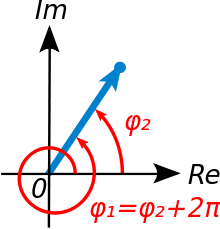
\includegraphics[scale=0.8]{dilema.png}\\
	{\small Aqu\'i, $\varphi_2$ es el argumento principal}
\end{center}

\subsection{Representaci\'on Exponencial}
Al llegar hasta la forma polar hemos dado un gran salto para adelante, uno que se completa agregando a todo lo visto hasta ahora una f\'ormula m\'as... una que nos dio nuestro querido amigo Leonard Euler: la \textbf{F\'ormula de Euler}
$$e^{i\theta} = \cos \theta + i\cdot \sin \theta$$

Tomando esto en consideraci\'on, y trabajando la forma polar anterior, llegamos a la c\'uspide de las distintas formas de representar n\'umeros complejos. He aqu\'i la \textit{forma exponencial}:
%	$$z = r (\cos \theta + i \sin \theta)$$
\begin{empheq}[box={\mybluebox[5pt]}]{equation*}
	\mbox{ \large $z = r e^{i\theta}$}			
\end{empheq}

Con esta forma de escribir complejos, se nos simplifica a\'un m\'as las operaciones de multiplicaci\'on y divisi\'on. Observa...

Si $z_1, z_2 \in \mathbb{C}$, con $z_1 = r_1e^{i\theta_1}$ y $z_2 = r_2e^{i\theta_2}$, entonces:
\begin{empheq}[box={\mybluebox[5pt]}]{equation*}
	\mbox{ \large $z_1 \cdot z_2 = r_1\ r_2\ e^{i(\theta_1+\theta_2)}$}			
\end{empheq}
\begin{empheq}[box={\mybluebox[5pt]}]{equation*}
	\mbox{ \large $\displaystyle \frac{z_1}{z_2} = \frac{r_1}{r_2}\ e^{i(\theta_1-\theta_2)}$}			
\end{empheq}

E inclusive nos habilita algo que hasta ahora no nos atrevimos hacer con los n\'umeros complejos (sino s\'olo con $i$): definir la potenciaci\'on en $\mathbb{C}$. Tenemos que la potenciaci\'on de complejos es as\'i de simple si se los representa en su forma exponencial:
\begin{empheq}[box={\mybluebox[5pt]}]{equation*}
	\mbox{ \large $z_1^n = (r_1e^{i\theta_1})^n = r_1^n\ e^{i(n\theta_1)}$}			
\end{empheq}

Con esto, llegamos al mismo resultado que otro de nuestros amigos matem\'aticos, De Moivre, con su \textbf{F\'ormula de De Moivre}:
$$(\cos \theta + i \sin \theta)^n = \cos (n\theta) + i \sin (n\theta)$$

Recordando que el argumento de un complejo puede tener infinitos valores que difieran en $2\pi$, la forma gen\'erica de representaci\'on en forma exponencial ser\'ia:
\begin{empheq}[box={\mybluebox[5pt]}]{equation*}
	\mbox{ \large $z = r e^{i(\theta + 2k\pi)}$, con $k \in \mathbb{Z}$	}		
\end{empheq}

Este peque\~no hecho que puede pasar f\'acilmente por desapercibido no ha de ser pasado por alto. Ya que nos es de gran importancia para casos como el que sigue: si elev\'asemos un complejo a un exponente racional de la forma $\frac{1}{n}$, con $n \in \mathbb{Z}$, y aplic\'asemos la f\'ormula de De Moivre, probablemente nos contentar\'iamos con haber encontrado la $n$-\'esima ra\'iz de nuestro complejo, pero la historia no acaba all\'i en absoluto. Pues observen c\'omo, para distintos $k$ considerados, al dividirlos por $n$, otro entero, no necesariamente dar\'an otro n\'umero entero. Si el cociente $\frac{k}{n}$ no es entero, entonces el t\'ermino $2k\pi$ que antes se le sumaba indiferentemente al argumento principal, ahora \textit{no} arrojar\'a valores congruentes. Con ello quiero decir que para distintos $k$, en el c\'alculo de la $n$-\'esima ra\'iz, tendr\'iamos resultados diferentes. La cantidad de ra\'ices diferentes que obtendr\'iamos ser\'ia igual al \'indice de la ra\'iz considerada ($n$).

Lo verifiquemos:
{\large
\begin{eqnarray*}
z^{1/n} &=& \left[r\ e^{i(\theta + 2k\pi)}\right]^{1/n}\\
&=& \sqrt[n]{r}\ e^{i (\frac{\theta}{n} + \frac{2k\pi}{n})}
\end{eqnarray*}
}
Donde $\displaystyle \frac{2k\pi}{n}$ con $k, n \in \mathbb{Z}$ adoptar\'a $n$ valores distintos con $k$ variando desde 0 hasta $n-1$. Para valores enteros de $k$ fuera de ese rango se volver\'an a obtener c\'iclicamente las primeras $n$ ra\'ices calculadas.

\begin{multicols} {2}
Analizando los resultados, vemos que todas las ra\'ices de un complejo tienen entre s\'i el mismo m\'odulo, pero difieren en su argumento. Esto nos quiere decir que... est\'an distribuidos todos en torno a una circunferenci de radio $\sqrt[n]{r}$ en torno a $z=0$, y se localizan equitativamente espaciados de tal manera que el \'angulo subtendido entre dos ra\'ices consecutivas es de $\displaystyle \frac{2\pi}{n}$.
\begin{center}
	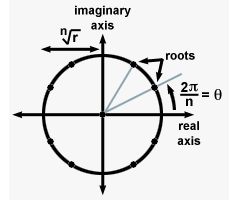
\includegraphics[scale=1.2]{roots.png}
\end{center}
\end{multicols}

\section{Reflexi\'on sobre lo aprendido}
En fin, ?`los n\'umeros son para contar?

\end{document}